\documentclass{article}
\usepackage{graphicx} % Required for inserting images
\usepackage{parskip}
\usepackage{float}
\usepackage{hyperref}
\usepackage{multirow}
\usepackage{rotating}
\usepackage{fourier} 
\usepackage{array}
\usepackage{makecell}

\renewcommand\theadalign{bc}
\renewcommand\theadfont{\bfseries}
\renewcommand\theadgape{\Gape[4pt]}
\renewcommand\cellgape{\Gape[4pt]}

\title{DevOps Project}
\author{Dagmara Przygocka\\Petroula Stamou
\\Szymon Gałecki\\Marcus Gunnebo}
\date{May 2023}

\begin{document}

\maketitle

\section{System's Perspective}
    \subsection{Design and architecture (Petroula)}
        MiniTwit, a legacy application, was assigned to our team with the goal of refactoring it and modernizing it with up-to-date technologies and practices. After careful consideration, the team made the decision to leverage Python with the Django framework. \\
        The system follows a container-based architecture, where each component is encapsulated within its own Docker image. The application itself is implemented in Python using the Django framework, while the API is developed using FastAPI. Both components rely on Postgres as database.\\
        For effective logging, the team opted to utilize the EFK stack, consisting of Elasticsearch, Filebeat, and Kibana. Nginx was employed as reverse proxy within the network. This setup ensures comprehensive log management and analysis capabilities.\\
        In terms of monitoring, Prometheus was chosen as the tool to gather metrics and monitoring data from the system. Grafana was then employed to visualize this data, allowing for effective monitoring and analysis of system performance and health.\\
        By adopting these technologies and practices, the team was able to modernize MiniTwit, enhancing its functionality, scalability, and maintainability while leveraging their existing Python expertise and expanding their knowledge in new frameworks and tools. \\
        Furthermore, we have prepared Context UML diagram and a Deployment UML diagram to provide a visual representation of our architectural solution.
        \begin{figure}[H]
            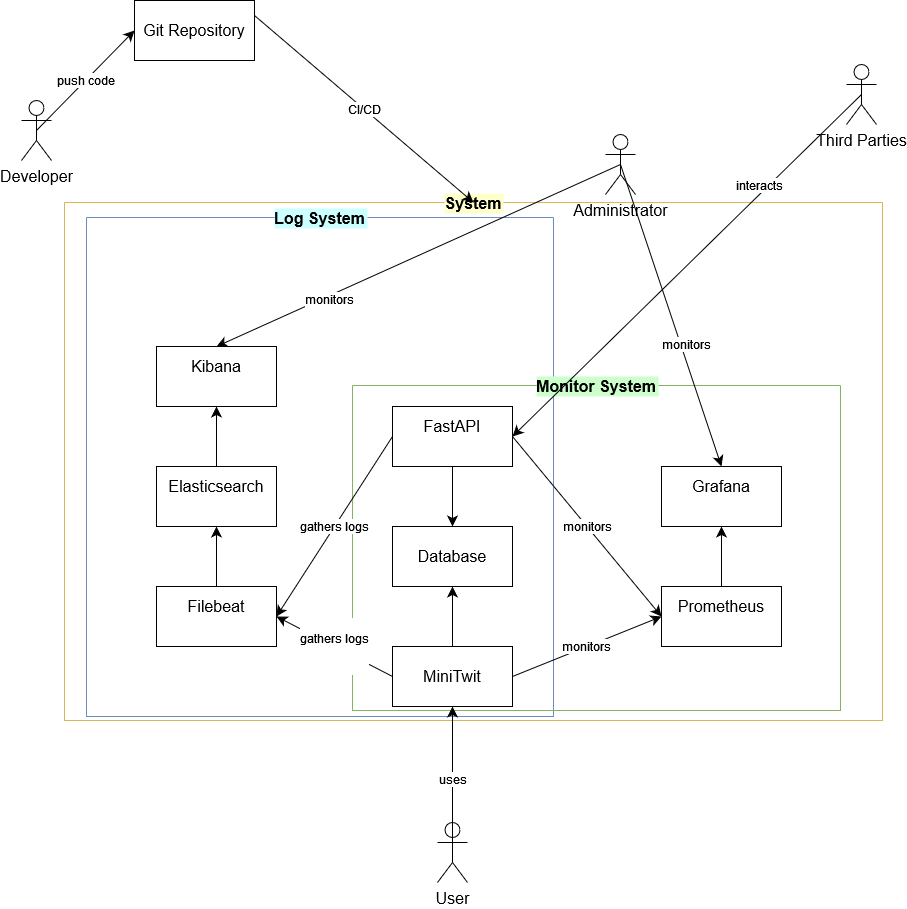
\includegraphics[width=13cm]{images/Context.png}
            \centering
            \caption{Context UML diagram}
            \label{fig:Context}
        \end{figure}
        \begin{figure}[H]
            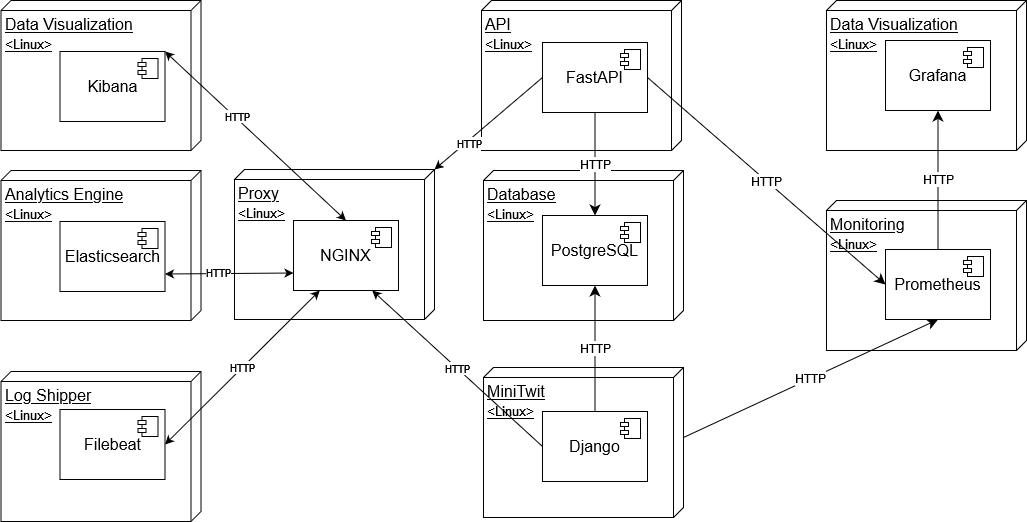
\includegraphics[width=13cm]{images/Deployment.png}
            \centering
            \caption{Deployment view}
            \label{fig:Deployment}
        \end{figure}
    \subsection{Dependencies (Petroula)}
        \begin{itemize}
            \item \textbf{Django} for the APP.
            \item \textbf{FastAPI} for the API implementation.
            \item \textbf{PostgreSQL} as for the database of the system.
            \item \textbf{GitHub} for hosting code base and CI/CD pipelines.
            \item \textbf{Digital Ocean} to host the application.
            \item \textbf{Vagrant} to build the droplet in Digital Ocean.
            \item \textbf{Docker} and \textbf{DockerHub} for Containerization and hosting the images of the system.
            \item \textbf{Prometheus} For monitoring the application and API
            \item \textbf{Grafana} for visualizing the monitoring data
            \item \textbf{EFK stack} for gathering the logs, analysing and visualizing them. 
            \item \textbf{Nginx} as reverse proxy.
        \end{itemize}
    \subsection{State of your systems (Petroula)}
        The application is running without errors and it will continue to run until 15/6/2023 on \href{http://138.68.73.127:8000}{http://138.68.73.127:8000}. The code can be found in \href{https://github.com/szymongalecki/ITU-MiniTwit}{ITU-MiniTwit}. Our system managed to handle 12,150,558 requests during the simulation.
    \subsection{License (Petroula)}
        Our intention is not to profit from this project; therefore, we have chosen to release the code under the MIT License.
    \subsection{Weekly Tasks (Petroula)}
        \subsubsection{Week 2: Refactor ITU-MiniTwit in another programming language and tech. stack}
            We choose to transition to Django from Flask and utilized FastAPI.\\
            More information can be found in the correspondent section.
        \subsubsection{Week 3: Deployment to a remote server.}
            We utilized Digital Ocean a cloud-based infrastructure provider to deploy our application.\\
            More information can be found in the correspondent section.
        \subsubsection{Week 4: Setup CI \& CD for reproducible builds, tests, delivery, and deployment }
            The team chose a cloud-based CI/CD solution, GitHub Actions. The CI/CD pipeline is configured in continuous-deployment.yml, triggering on main branch pushes and allowing manual triggers.\\
            More information can be found in the correspondent section.
        \subsubsection{Week 6: Monitoring}
            We added Prometheus and Grafana to our system for improved monitoring and visualization.\\
            More information can be found in the correspondent section.
        \subsubsection{Week 7: Test suite and static code analysis}
            We utilized Django Unit Tests in our project to ensure the correct functionality of our application. In addition to unit tests, we also employed five static analysis tools for our project: Flake8, Black, and Bandit, sonarcloud, codeclimate.\\
            More information can be found in the correspondent section.
        \subsubsection{Week 8: Logging, and Log Analysis. Service-level agreements.}
            The team chose to implement the EFK (Elasticsearch, Filebeat, Kibana) stack for Docker logging and Nginx for reverse proxy. This setup provides secure access to Elasticsearch and Kibana with authentication. The logging can be accessed at\\ \href{http://138.68.73.127:5000/app/home}{http://138.68.73.127:5000/app/home}. using the provided credentials.\\
            More information can be found in the correspondent section.
        \subsubsection{Week 9: Security Assessment \& Pen Testing}
            During the risk identification and analysis process, assets such as the web application, API, Docker Hub, GitHub repository, Digital Ocean, and monitoring tools were identified. Threat sources like SQL injection, Cross-Site Scripting (XSS) attacks, Denial of Service (DoS) attacks, password leakage, exposure of hard-coded passwords, unused open ports, and vulnerabilities in frameworks or Docker images were considered. Risk scenarios were constructed based on these threats.\\
            More information can be found in the correspondent section.
        \subsubsection{Week 10: Scaling}
            The team decided to implement a replication strategy and an Infrastructure as a Service (IaaS) setup for the project. The replication strategy involved creating a high-availability setup with a hot and standby server for the ITU-MiniTwit application. \\
            More information can be found in the correspondent section.
    
\section{Process' perspective}
\subsection{Team organization and development (Dagmara)}
%\begin{itemize}
%\item (D) How do you interact as developers?
%\item (D) How is the team organized?
%\item (D) Applied branching strategy.
%\item (D) Applied development process and tools supporting it
%For example, how did you use issues, Kanban boards, etc. to organize %open tasks
In our development team all members had equal roles and responsibilities. Each task was evaluated at our weekly meeting and assigned to one or two team members according to their preferences. This allowed team members to contribute to the project in areas they were most interested in and eager to learn.
\par

\noindent The development process of the MiniTwit application revolved around two main platforms GitHub and Teams. The GitHub platform served as code storage, running CI/CD pipelines and maintaining the list of issues that needed to be completed. Each week, new issues were created upon receiving new assignments to ensure proper organization and updates of the tasks. On the other hand, the Teams platform was mainly used for communication, meeting notes and requests for a review of the pull requests.
\par

\noindent To establish clear guidelines in file CONTRIBUTE.md for contributions to the project. The team outlined rules regarding branching, merging and GitHub workflow. 

The file can be found at this \href{https://github.com/szymongalecki/ITU-MiniTwit/blob/main/CONTRIBUTE.md}{link}.

\subsection{Repository organization (Dagmara)}
%item (D) Organization of your repositor(ies).
%That is, either the structure of of mono-repository or organization of artifacts across repositories.
%In essence, it has to be be clear what is stored where and why.
The repository mostly consists of the folders with names which represents services ran in our setup. This structure allowed our team to easily find and make changes to the code. The folders are:

\begin{itemize}
  \item \texttt{./github/workflows}: This folder contains pipelines, including one for deployment to the Digital Ocean droplet and another for checking quality gates for each pull request.
  
  \item \texttt{ITU\_MiniTwit}: This folder contains the code for the MiniTwit application, developed using Python Django.The project contains the application's behavior, manage data models and handle HTTP requests. The folder also includes Docker file for building image called "minitwitimage" used in docker-compose file.(in remote\_files folder)
  
  \item \texttt{ITU\_MiniTwitFlask}: This folder contains the code for the old MiniTwit application, written with Python Flask. Kept for references and historical purposes.
  
  \item \texttt{Minitwit\_api}: This folder contains a set of APIs that enable communication between external services and the MiniTwit application. In addition, it holds Docker file for building "apiminitwit" image used in docker-compose file.(in remote\_files folder)
  
  \item  \texttt{prometheus}, \texttt{grafana}, \texttt{filebeat}, \texttt{nginx}, and \texttt{Database}: Folders for other services where each contains Docker file, configuration files and necessary code for building the image used in docker compose file in the deployment process.
  
  \item \texttt{dev\_notes} and  \texttt{docs}: These folder contain development notes/documentation with reasoning behind chosen technology, SLA (Service Level Agreement), or postmortem tasks.
  
  \item \texttt{remote\_files}: This folder contains files copied to the Digital Ocean droplet during its creation.
  
  \item \texttt{saved\_objects}: This folder contains Kibana configurations that can be loaded into a new environment setup to reuse dashboards, indexed patterns, filters, and visualizations.
  \item \texttt{hot\_server}: This folder contains Vagrant configurations that can be used for creating a new environment with main and backup server.
\end{itemize}
Additionally, the repository includes the following files:

\begin{itemize}
  \item Quality gates tools configuration files: \texttt{.flake8}, \texttt{bandit.yml}, \texttt{pyproject.toml}.
  
  \item \texttt{Vagrantfile} for automated droplet creation.
  
  \item \texttt{docker-compose} file for spinning up Docker containers, networks, and volumes for local development.
  
  \item \texttt{README.md} project description file.
  
  \item \texttt{CONTRIBUTE.md} contains rules for contributing to the project.
  
  \item \texttt{.gitignore} file lists directories and files to ignore when pushing code to the repository.
\end{itemize}
\subsection{CI/CD description (Dagmara)}
%\item (D) A complete description of stages and tools included in the CI/CD chains.
%That is, including deployment and release of your systems.
In the project, we decided to create three GitHub Actions: first for deploying the project to a Digital Ocean droplet on the main branch, second for extended version of the first one with rolling updates and last one for performing quality checks on the code in each pull request before merging it into the main branch. The file containing the deployment pipeline is set up as follows:
\begin{enumerate}
\item \textbf{Trigger}
The workflow is triggered every time there is a push to the main branch. Additionally, we allow for manual triggering of the workflow.

\item \textbf{Jobs}
\begin{enumerate}
    \item \textbf{Build}: The workflow is set to run on an environment with the latest stable version of Ubuntu.

\item \textbf{Steps}
\begin{enumerate}
    \item \textbf{Checkout to the repository}: This step allows the workflow to access the source code and files in the repository.
    \item \textbf{Setup Python 3.10}.
    \item \textbf{Install Black, Bandit, Flake8}, and the necessary requirements for MiniTwit\_api and ITU\_MiniTwit.
    \item \textbf{Run Black, Bandit}, and Flake8 quality gate tools.
    \item \textbf{Login to Docker} using environmental variables for the password and username with a pre-built action.
    \item \textbf{Setup Docker Buildx} with a pre-built action: This allows for building images for multiple architectures and platforms from a single build context, as well as providing advanced caching and build parallelism features.
    \item \textbf{Build and push the Minitwitimage, Minitwit API, database, Grafana, Prometheus, and Nginx to Docker Hub}. The image is built using the Dockerfile of the service and includes the Docker username of the person whose Docker Hub we will use for the project. Building and pushing new images to Docker Hub allows us to have images with the latest changes made to those services.
    \item \textbf{Build and run the MiniTwit test}. The step checks if all tests for ITU\_MiniTwit app passed. As of this moment there is an error encountered, so we allow this step to fail without stopping the deployment flow.
    \item \textbf{Configure SSH}.The SSH configuration step creates a folder called ".ssh" and adds the private SSH key used to communicate with Digital Ocean. The corresponding public key is registered on Digital Ocean, allowing the GitHub Action to deploy the changes.
    \item \textbf{Deploy to server}.The Deploy to server step uses the private SSH key to SSH into the server hosted on Digital Ocean. It runs the "deploy.sh" script in the 'minitwit' folder on the virtual machine, which pulls the new images from Docker Hub and runs the "docker-compose.yml" file.
\end{enumerate}
\end{enumerate}
\end{enumerate}
The second pipeline adds to the one described before steps that check if the deployment is successful. If that is the case it deploys the changes to the backup server. Last pipeline uses a subset of the deployment GitHub action, which includes checks for the quality of the code.


%\item (M) How do you monitor your systems and what precisely do you monitor?
\subsection{Monitoring (Marcus)}
\subsubsection{Prometheus and Grafana}
We are monitoring our system using two services: Prometheus and Grafana. The package Prometheus FastAPI Instrumentator in the API is responsible for sharing metrics about the APIs endpoints, which Prometheus views on the sub page \textit{metrics}. Grafana then collects these metrics from Prometheus with a 15 second interval and displays them on four different dashboards. Grafana visualizes the number of requests and responses for each endpoint, and also shows whether it is connected to Prometheus. The Prometheus image was pulled from the Prometheus Docker hub and supplied with a configuration file, while the Grafana image was built locally and uploaded to Docker hub. All the images currently used in the docker-compose are available on our Docker hub.

\subsubsection{Prometheus}
For monitoring we used Prometheus. It is a monitoring system used for scraping metrics from a wide variety of sources, including for our case an API. It is designed to be reliable, efficient, and highly scalable, allowing developers to easily monitor their own applications. We have used it to collect metrics for Grafana, to further analyze and visualize the data. It is also open source and free for anyone to use. We used a package to implement it that was specifically designed for FastAPI. 

\subsubsection{Grafana}
For creating dashboards we used Grafana. It is an open source data visualization and monitoring platform used for creating dashboards and graphs. It can be used for a variety of applications, such as monitoring and alerting and for displaying real-time data from sources such as for us, Prometheus. Grafana allows users to explore their data, visualize their metrics, and gain insights into their data.

\subsubsection{Dashboard}
Grafana was manually configured at first, by creating four different dashboards to the specific needs of our project. The configuration was then exported as a JSON file, and then used to enable automatic set up each time the application is deployed. This also includes setting up a user with username and password given by the teachers in the course. This streamlines the process of monitoring endpoints in the API, decreasing the amount of manual tasks required.

    \subsection{Logging (Petroula)}
        In our configuration, Filebeat is set up to collect logs specifically from Docker containers residing in the /var/lib/docker/containers directory. However, we narrow our focus to only gather logs from two specific containers: the APP and API containers. Within the APP container, we capture Django logs pertaining to the requests made, as well as the system state. As for the API container, we collect logs related to both POST and GET requests, including the corresponding responses. Additionally, we capture the system states for both containers, providing valuable insights into the overall functioning of the system.\\
        The team has made strategic decisions to create a set of informative visualizations. These visualizations include the following metrics:
        \begin{itemize}
            \item Total number of logs for each container, enabling us to gauge the logging activity within individual containers.
            \item Logs categorized by API, APP, and general sources, providing insights into specific components and overall system behavior.
            \item An analysis of the number of requests based on the HTTP methods used, namely POST, GET, and DELETE, highlighting the distribution of different request types.
            \item The count of log levels, such as error, info, debug, and warning, enabling us to assess the severity and prevalence of different log events.
        \end{itemize}
        By visualizing these key metrics, we gain a comprehensive overview of the logging activity, application components, request patterns, and log severity levels, empowering us to make data-driven decisions and effectively troubleshoot any issues within the system.\\
        You can find more detailed information about logging in the following link:  \href{https://github.com/szymongalecki/ITU-MiniTwit/blob/main/dev_notes/logging.md}{ELK}
\subsection{Security assessment (Petroula)}
	\subsubsection{Risk Identification}
	\paragraph{Identify assets}
	\begin{itemize}
		\item Web application
		\item Docker Hub
		\item Github repository
		\item Digital Ocean
		\item Grafana / Prometheus / Kibana
	\end{itemize}
	\paragraph{Identify threat source}
	\begin{itemize}
		\item SQL injection 
		\item Cross-Site Scripting (XSS) attacks
		\item Denial of Service (DoS) attacks
		\item Exposure of hard-coded passwords in public repositories (e.g., GitHub)
		\item Unused open ports
		\item Administrator’s passwords and their strength on all relevant platforms
		\item Vulnerabilities in frameworks or docker images used
	\end{itemize}
	\paragraph{Construct risk scenarios}
	\begin{itemize}
		\item Attacker performs SQL injection attack on the application to download, alter, or delete sensitive data.
		\item Attacker uploads a malicious script as a comment, which can affect the system when loaded by the application, potentially causing harm or enabling further attacks.
		\item Denial of Service (DoS) attack renders the system unavailable to users.
		\item Developer mistakenly uploads hard-coded passwords for administrator accounts
	\end{itemize}

	\subsubsection{Risk Analysis}
	\paragraph{Determine likelihood}
	\begin{itemize}
		\item The likelihood of encountering a \textbf{SQL injection} vulnerability in our application is minimal to none. We have thoroughly reviewed the app and identified only three forms that an attacker could potentially exploit: the login and registration forms, as well as the post message form. 
		\item The likelihood of \textbf{XSS attacks} within our application remains minimal.
		\item 	Our application is hosted on DigitalOcean, which offers robust \textbf{DDoS} protection mechanisms and network security features.
		\item The scenario of \textbf{password leakage} is highly unlikely due to our robust security measure in place. Secure password storage: All passwords are meticulously stored in the database using a strong hashing algorithm combined with the utilization of salt. 
		\item \textbf{Hard-coded passwords exposed} in public repositories pose a potential risk due to human error. Although we strive to maintain strict security practices, the possibility of such occurrences cannot be completely ruled out. 
		\item The presence of \textbf{unused open ports} is an improbable scenario as our application meticulously manages its port configurations. We maintain a strict policy of only opening and monitoring specific ports that are essential for the application's functionality.
		\item The potential \textbf{compromise of administrator password}s is a valid concern, considering the shared nature of these credentials. As part of our operational procedures, administrator passwords were shared within either the lecture GitHub repository or our own GitHub repository. 
		\item The likelihood of \textbf{vulnerabilities in frameworks or Docker images} utilized in our system is a valid concern. With a diverse range of dependencies, the potential for vulnerabilities does exist.  dependencies.
	\end{itemize}
	\paragraph{Determine impact}
	\begin{itemize}
		\item SQL injection: Moderate
		\item Cross-Site Scripting (XSS) attacks: Severe
		\item Denial of Service (DoS) attacks: Significant
		\item Password leakage: Severe
		\item Exposure of hard-coded passwords: Severe/Negligible
		\item Unused open ports: Significant
		\item Administrator’s passwords Severe/Negligible
		\item Vulnerabilities in frameworks or docker images used: Moderate
	\end{itemize}
	\paragraph{Discuss what are you going to do about each of the scenarios}
	\begin{itemize}
		\item SQL injection\\
		Users should be notified immediately via emails in the event of personal information leakage. It's important to inform the users that their passwords are securely stored, utilizing hashing techniques instead of plain text.
		\item Cross-Site Scripting (XSS) attacks\\
		To effectively address the attack, the website should go temporarily offline or restrict access to it until the issue is resolved. Furthermore, it is crucial to promptly notify all affected users and provide them with guidance on changing their passwords, while encouraging them to remain vigilant against any malicious activities.
		\item Denial of Service (DoS) attacks\\
		We are using monitoring tools like Prometheus to detect unusual patterns or sudden spikes in network traffic in order to identify and respond to a potential DoS attack in real time.
		\item Password leakage\\
		The stored password are in hashed form but nevertheless the affected users will be notified and will be prompt to change their passwords. 
		\item Exposure of hard-coded passwords\\
		Upon finding any such password the developers should immediately change the compromised password and assess the system for possible security issues.
		\item Unused open ports\\ 
		Any open port to the system should be closed immediately after discovery, and assess any possible security bridges.
		\item Administrator’s passwords\\
		All administrator pages should use two factor authentication in combination with strong passwords.
	\end{itemize}
	\paragraph{Use a Risk Matrix to prioritize risk of scenarios}
	\begin{table}[!h]
		\centering
		\begin{tabular}{|c|c|c|c|c|c|c|}
			\hline & & \multicolumn{5}{| c |}{Impact}\\
			\cline{3-7}&& Negligible & Minor & Moderate & Significant & Severe\\
			\hline \multirow{15}{*}{\begin{sideways}Likelihood\end{sideways}} & Very Likely&&&&&\\
			\cline{2-7}&Likely&\thead{Exposure \\of hard-coded \\passwords}&&&&\\
			\cline{2-7}&Possible&&&\thead{frameworks or \\docker images} &&\\
			\cline{2-7}&\multirow{2}{*}{Unlikely}&&&\multirow{2}{*}{\textbf{SQL injection}}&\thead{Unused \\open ports}&\thead{Password\\leakage} \\
			\cline{6-7}&&&&&\textbf{DDOS}&\thead{Cross-Site\\Scripting\\(XSS)}\\
			\cline{2-7}&Very Unlikely&\thead{Administrator’s \\passwords strength} &&&&\\
			\hline 
		\end{tabular}
	\end{table}
 \newpage
	\subsubsection{Pen-Test Your System}
    During our Pen-Test, we initiated the assessment by employing the nmap command with the flags -v -A -sV -Pn. This allowed us to identify any open ports that might pose a threat to our system. As anticipated, the scan revealed only the intended open ports, all of which were diligently monitored by Prometheus to ensure system security.\\
	Next, we proceeded to execute the OWASP ZAP 2.12.0 tool on our website, which provided us with a comprehensive list of vulnerabilities requiring attention. This allowed us to prioritize our tasks and address each vulnerability accordingly. Please refer to Figure 3 for the complete list, with alert levels ranging from medium priority to information.\\
	For the final phase, we conducted targeted attacks on our application using custom scripts and various scenarios, such as SQL injections and XSS attacks. Through this process, we identified a key vulnerability that demanded\\ immediate attention: cross-site scripting attacks. To fortify our application, we implemented CSRF tokens in all forms susceptible to this vulnerability, thus enhancing the overall security of our app.
 \begin{figure}[H]
		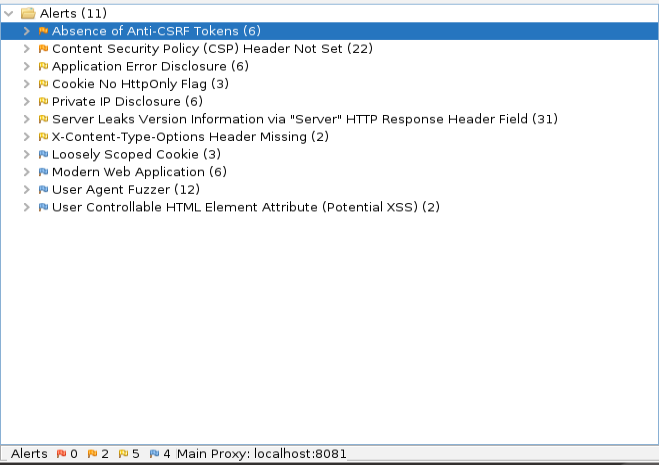
\includegraphics[width=12cm]{images/Screenshot_3.png}
		\centering
		\caption{OWASP ZAP Alerts}
		\label{fig:alerts}
	\end{figure}
 You can find a more thorough analysis in the following link \href{https://github.com/szymongalecki/ITU-MiniTwit/blob/main/dev_notes/Penetration%20Test%20Assesment.md}{Penetration Test Assessment.md}
\subsection{Applied strategy for scaling and load balancing (Dagmara)}
The team decided to scale the project by implementing a high-availability setup with a hot and standby server for our ITU-MiniTwit application. The set up includes having two replicas of our MiniTwit application server where only one is ever active at a time. To implement it we followed Digital Ocean tutorial: How To Set Up Highly Available Web Servers with Keepalived and Reserved IPs on Ubuntu 14.04 (\href{https://www.digitalocean.com/community/tutorials/how-to-set-up-highly-available-web-servers-with-keepalived-and-reserved-ips-on-ubuntu-14-04}{link}).

The current status of MiniTwit application includes running database service as a part of docker-compose stack. Each server has its own stack deployed which includes volumes where the data are kept. The result of this implementation is that no matter which approach we will take, either Docker Swarm or High Availability setup with a hot and standby server, we will have the problem with data consistency. The reason why we chose the second approach is due to our Digital Ocean account which allows only 3 droplets where one was already taken by the initially deployed server. In order to create replicas we would need to take down the current server which would result in loss of volumes we collected when the simulation was running. Future improvements could include:
\begin{itemize}
\item Separating databases form the stack so all replicas could have one source of data.
\item Increasing Digital Ocean account resources so we could have more than 3 droplets.
\item Migrating the data from the initial server and deploying the replicas.
\end{itemize}
Due to the characteristics of the implemented replication, no load balancing was included into the architecture design.
More information can be found in the document called Replicas \_and\_IaaS.md (\href{https://github.com/szymongalecki/ITU-MiniTwit/blob/replication/dev_notes/Replicas%20_and_IaaS.md}{link}).

\subsection{AI-assistants (Marcus)}
During the project we have utilized AI-assistants for two reasons. For debugging docker files and rewriting text for development notes. It has never been used to produce any code, which could be interesting for a future project. But for us, where the emphasis has been to learn new systems and frameworks during this project, we argued that it would probably hinder us in getting a solid understanding if code was generated.

\subsubsection{Debugging}
When working with a new framework, a big part of learning it comes down to reading documentation and searching for information online. So during our project we have used Chat-GPT as a search tool to get a better understanding of our code. We have used it to get an explanation for arguments and variables used in docker files. This was done to get a more exact explanation and to get an answer faster, which have worked pretty well. It is not possible to use Google in the same way for extracting an answer specific to our code. An example for when Chat GPT was used to extract information for debugging a docker file can be seen in Figure \ref{fig:gptdebugging}.

\begin{figure}[H]
    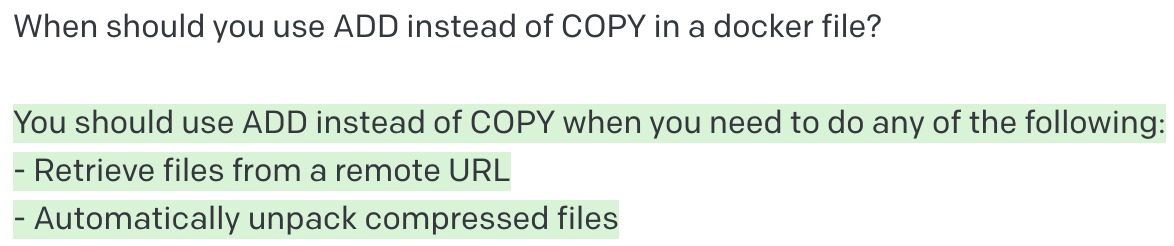
\includegraphics[width=10cm]{images/gptdebugging.png}
    \centering
    \caption{Chat GPT used for debugging docker files}
    \label{fig:gptdebugging}
\end{figure}

\subsubsection{Rewriting}
After completing tasks during this project it has been vital to produce good development notes for the rest of the group. This is because an overall understanding of the system creates a better opportunity to develop new features. Due to the fact that we are four students from four different countries where non has English as a first language, we used AI-assistants to produce better written documentation for our project. The most important part have been to give it a good prompt containing all important information and to thoroughly read through the suggested rewrite to make sure it is correct. There is always a risk that the model makes a qualified guess, that ends up being not true. An example for how we could have used Chat GPT for rewriting development notes can be seen in Figure \ref{fig:gtprewrite}.

\begin{figure}[H]
    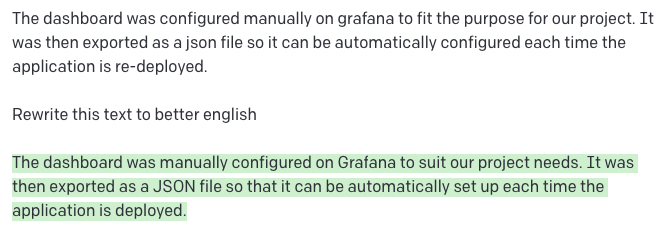
\includegraphics[width=10cm]{images/gptrewrite.png}
    \centering
    \caption{Chat GPT used for rewriting development notes}
    \label{fig:gtprewrite}
\end{figure}

There is always a risk using AI-assistants due to the fact the they sometimes generate wrong answer or even lies. But there are use cases where we see a great benefit to using them.

\section{Lessons Learned Perspective (Szymon)}
% Describe the biggest issues, how you solved them, and which are major lessons learned with regards to:
% \begin{itemize}
% \item evolution and refactoring
% \item operation, and
% \item maintenance
% \end{itemize}
% of your ITU-MiniTwit systems. Link back to respective commit messages, issues, tickets, etc. to illustrate these.

% Also reflect and describe what was the "DevOps" style of your work. For example, what did you do differently to previous development projects and how did it work?

\subsection{Evolution and refactoring issues}
In the beginning of the project we realized that no one had any front-end experience. Most of us were familiar with Python so we decided to refactor application to popular and well documented framework - Django. Initial workload was divided into three parts: "refactor application to Django", "find out what is Docker and how to use it", "learn what is API and build it". After two weeks we had all the components: application, API and Dockerfile for containerization. Most of the problems became visible during integration.
\begin{itemize}
    \item Application used models, built-in Django ORM solution, to represent tables of original schema. However, the resulting schema created from Django models was different from the original one.
    \item Application had to create its own database in order to function.
    \item API was built to use original schema.
\end{itemize}
To mitigate this problem quickly we prioritized API as the simulator was soon supposed to start. We packed everything into a single container and deployed to Digital Ocean as PaaS. API processed requests and stored data in the SQLite database. Application had no access to data supplied by API and it worked as a separate standalone service. Additional problems emerged before we solved the old ones. 
\begin{itemize}
    \item Once container crashes all our is gone.
    \item We had no idea how to pull our data out of running container.
\end{itemize}
We didn't want the database to fully depend on application but at the same time we knew that it would be hard to remove models from Django logic. We were required to implement ORM which was satisfied by application but we wanted our database to run in a separate container. We decided that API will follow schema generated by Django and that data will be migrated using Django migration tools. We decided to use PostgreSQL image for our database, and that API and application will connect to it through a default network created by docker-compose.
\\
We managed to pull out data from Digital Ocean application using Netcat. Our application must have crashed because we were missing two weeks of data. We migrated data and run all services in separate containers using docker-compose.
\\
Lessons:
\begin{itemize}
    \item Agree and write down the main assumptions before starting work.
    \item Communicate changes and the process, inform team members.
    \item Do not wait until solution is perfect, focus on deploying small changes.
\end{itemize}

\subsection{Operation issues}
Every single change of the Vagrant file, such as adding a port, required rebuilding the VM. All updates to GitHub secrets were done manually but were rare. Changes to docker-compose file inside of VM were applied manually through console but were also rare, since we changed content of images way more often than added a new service.
\\\\
We didn't realize how good are the tools for assessing code quality and safety. Problems are not only found but also explained with examples.

Lessons:
\begin{itemize}
    \item Do not automate rare tasks just for sake of automation.
    \item Always use tools for code quality and safety, disallow merging branches with unsafe code using CI/CD pipeline.
\end{itemize}

\subsection{Maintenance issues}
We had lots of interesting maintenance issues. The first implementation of API failed local tests as it returned HTTP status code 204, after successful POST request, instead of code 200 specified in tests. We thought that this code was more adequate so we issued a PR on test file, which got merged.\\
Another interesting issue appeared after we redeployed. Status page for all groups showed that our API was not processing new requests. We expected to temporarily see value 0 on the latest\_ids graph as we didn't store value of latest in any way, but instead we saw 12. At this point we had no monitoring so we accessed API and checked that latest value is valid and that it's definitely not 12. After further investigation we concluded that it wasn't an error on our side but that status page must have been linked to the wrong address despite having updated it in repositories.py.\\
Last example worth mentioning is docker images compatibility. Teammates responsible for implementing monitoring were using Macbooks with ARM processors. They could use images built on x86 machines but not vice versa. During exercise session we build images using x86 machines and pushed them to secondary DockerHub account. Everything worked but we wanted to have all images on same DockerHub account. They were built again at home and suddenly Grafana started to expect Prometheus to send metrics over localhost:9090 instead of using default docker network. After building and testing local ARM images there was only one way to build images compatible with our VM. We integrated building images into CI/CD pipeline. They were successfully built and deployed but at the same time we tested on production.


\subsection{DevOps style}
One of the things that we didn't do before is required PR reviews before merging branch to main. It forced us to stay informed about the current state of the project. We also didn't write any developer notes before that course. When it comes to tasks, everyone picked up what they preferred and we had no fights over who takes what. This influenced future choices as we often preferred to work on the part that we were somewhat familiar with. Finally, our communication got better as project progressed.


\end{document}
